\documentclass[a4paper,11pt]{article}

    \usepackage{amsthm}

    %Use system fonts, only apply to XeTeX
    \usepackage{fontspec}
    \usepackage{xeCJK}

    \setmainfont[Ligatures={TeX}]{Minion Pro}
    \setsansfont[Ligatures={TeX}]{Myriad Pro}
    \setmonofont[Ligatures={TeX}]{Consolas}

    \setCJKmainfont[BoldFont=Adobe Heiti Std,ItalicFont=Adobe Kaiti Std,Ligatures={TeX}]{Adobe Song Std}
    \setCJKfamilyfont{kaiti}[Ligatures={TeX}]{Adobe Kaiti Std}
    \setCJKfamilyfont{sf}[Ligatures={TeX}]{Adobe Heiti Std}
    \setCJKfamilyfont{it}[Ligatures={TeX}]{Adobe Kaiti Std}
    \setCJKfamilyfont{tt}[Ligatures={TeX}]{Adobe Kaiti Std}

    \theoremstyle{definition}
    \newtheorem{exmp}{Example}[section]

    \usepackage{unicode-math}
    \unimathsetup{math-style=TeX}
    \setmathfont{XITS Math}

    %Adjust margin of document
    \usepackage{geometry}
    \geometry{left=2.5cm,right=2.5cm,top=2.5cm,bottom=2.5cm}

    \usepackage{listings}
    \usepackage{color}
    \definecolor{dkgreen}{rgb}{0,0.6,0}
    \definecolor{gray}{rgb}{0.5,0.5,0.5}
    \definecolor{mauve}{rgb}{0.58,0,0.82}

    \lstset{frame=tb,
    language={},
    aboveskip=3mm,
    belowskip=3mm,
    showstringspaces=false,
    columns=flexible,
    basicstyle={\small\ttfamily},
    numbers=none,
    numberstyle=\tiny\color{gray},
    keywordstyle=\color{blue},
    commentstyle=\color{dkgreen},
    stringstyle=\color{mauve},
    breaklines=true,
    breakatwhitespace=true,
    tabsize=3
    }

    \usepackage{spverbatim}

    \setlength{\parskip}{12pt}
    \setlength{\parindent}{0pt}

    % Graphics with mpost
    \usepackage{graphicx}
    \DeclareGraphicsRule{*}{eps}{*}{}

    % Hyperref in pdf
    \usepackage[usenames,dvipsnames,table]{xcolor}
    \usepackage{hyperref}
    \hypersetup{breaklinks,colorlinks,linkcolor=RoyalBlue,citecolor=red,urlcolor=purple,pdfstartview=FitH,pdfauthor={坂本ポテコ},pdftitle={XiaoTianQuan Setup Instructions}}

    \usepackage{xspace}



\begin{document}

\title{\Huge{XiaoTianQuan Setup Instructions}}
\author{坂本ポテコ}
\maketitle
\clearpage

\tableofcontents
\clearpage


{\Huge{Work In Progress.}}

\section{基本要求}

    本指南假定读者具备一定的SoC动手能力,能够简单识别电子元件能够安全的使用各种工具。

\subsection{硬件要求}

\subsubsection{服务器}

服务器需满足如下要求:

\begin{itemize}
  \item .Net Core 3.0支持平台(详见 \url{https://github.com/dotnet/core/blob/master/release-notes/3.0/3.0-supported-os.md})
  \item 可连接到闪电网络daemon (lnd) 的restful端点
  \item 可连接到SQL Server
  \item 可连接到Redis
  \item 可连接到Azure ServiceBus
  \item 售货机可及
\end{itemize}

Internet接入不是必须的。

\subsubsection{售货机}

售货机部分含有通用的交互控制板(含屏幕),以及机器特定的售货机控制板。



\section{服务器软件}

\subsection{安装}

请访问 \url{https://github.com/Andoromeda-Foundation/CryptoVendingMachineSoftware/releases} 以检索最新的服务器软件。

按照如下步骤安装并运行服务器软件,以下以 GNU/Debian Linux Buster 为例:

    \begin{enumerate}
        \item 准备一个全新并具有权限的 SQL Server数据库
        \item 准备一个Redis数据库
        \item 准备一台收款用、具备invoice权限的lnd,取得lnd的macroon,详见\ref{sec:lnd-macroon}
        \item 准备 Azure Service Bus 服务,我们会用到其中的队列服务
        \item 安装 .Net Core
        \item 下载并解压最新的服务器软件
        \item 配置服务器,详见 \ref{sec:server-config}
    \end{enumerate}

\subsection{Step by step}
    \subsubsection{SQL Server}
    为简化流程,建议用户使用Azure SQL database. 请参阅 \url{https://docs.microsoft.com/en-us/azure/sql-database/sql-database-single-database-get-started?tabs=azure-portal} 的用户指南。
    
    \subsubsection{Redis}
        \begin{lstlisting}
            $ # Install & start Redis
            $ sudo apt-get install redis-server
            $ sudo service redis-server start
        \end{lstlisting}

    \subsubsection{安装lnd}

请参照 \url{https://github.com/lightningnetwork/lnd/blob/master/docs/INSTALL.md} 提供的安装方法。

    \subsubsection{获取lnd macroon}\label{sec:lnd-macroon}

请使用如下命令获得macroon:

\begin{verbatim}
base64 [lnd config dir]/data/chain/[coin name]/[net name]/invoice.macaroon
\end{verbatim}


请将[]内的内容替换为相应字串。

    \begin{exmp}
    假定lnd配置文件在\verb|~/.lnd|下、使用\verb|bitcoin|并运行在\verb|simnet|上,则使用如下命令获得macroon,如图\ref{fig:show-macaroon}:
        \begin{verbatim}
        base64 ~/.lnd/data/chain/bitcoin/simnet/invoice.macaroon
        \end{verbatim}
    \end{exmp}

    \begin{figure}[htbp]
    \minipage[b][][b]{\textwidth}
        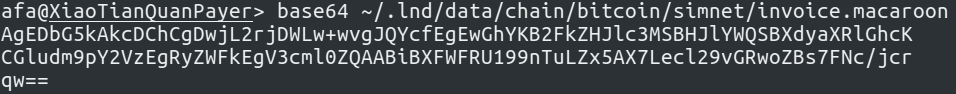
\includegraphics[width=\linewidth]{lnd-mac.png}
        \caption{显示 lnd macaroon}
        \label{fig:show-macaroon}
    \endminipage\hfill
    \end{figure}

请记录返回的字符串,字符串应当类似如下内容:
\begin{verbatim}
AgEDbG5kAkcDChCgFwjL2rjDWLw+wvgJQYcfEgEwGhYkw2FkZHJlc3MSBHJlYWQSBXdyaXRlGhcK
CGludm9pY2VzEgRyZzFkEgV3cml0ZQAABiBXFdpRU199nTuLZx5AX7Lecl29vGRwoZBs7FNc/jcr
qw==
\end{verbatim}

    \subsubsection{Azure ServiceBus}
请参阅 \url{https://docs.microsoft.com/en-us/azure/service-bus-messaging/service-bus-quickstart-portal} 以创建一个Azure ServiceBus. 在Create a queue in the Azure portal步骤中,请参阅指南,创建如下四个queue:
\begin{itemize}
  \item VendingMachineUnlock
  \item PaymentExpiry
  \item ProductUnfulfilledRefund
  \item PendingLightningNetworkInvoice
\end{itemize}
    
    \subsubsection{安装.Net Core}
    请参考 请参考 \url{https://dotnet.microsoft.com/download/linux-package-manager/debian10/runtime-current} 以安装 .Net Core Runtime
    
    \subsubsection{安装服务器}
    
        \begin{lstlisting}
$ # Install server
$ wget \ https://github.com/Andoromeda-Foundation/CryptoVendingMachineSoftware/releases/download/1.0.0-alpha/server.tar.gz
$ tar xf server.tar.gz
        \end{lstlisting}

\subsection{服务器配置}\label{sec:server-config}

服务器软件目录内含有\verb|appsettings.json|, 文件如图\ref{fig:appsettings},包含如下需要编辑/修改的section:

    \begin{figure}[htbp]
    \minipage[b][][b]{\textwidth}
        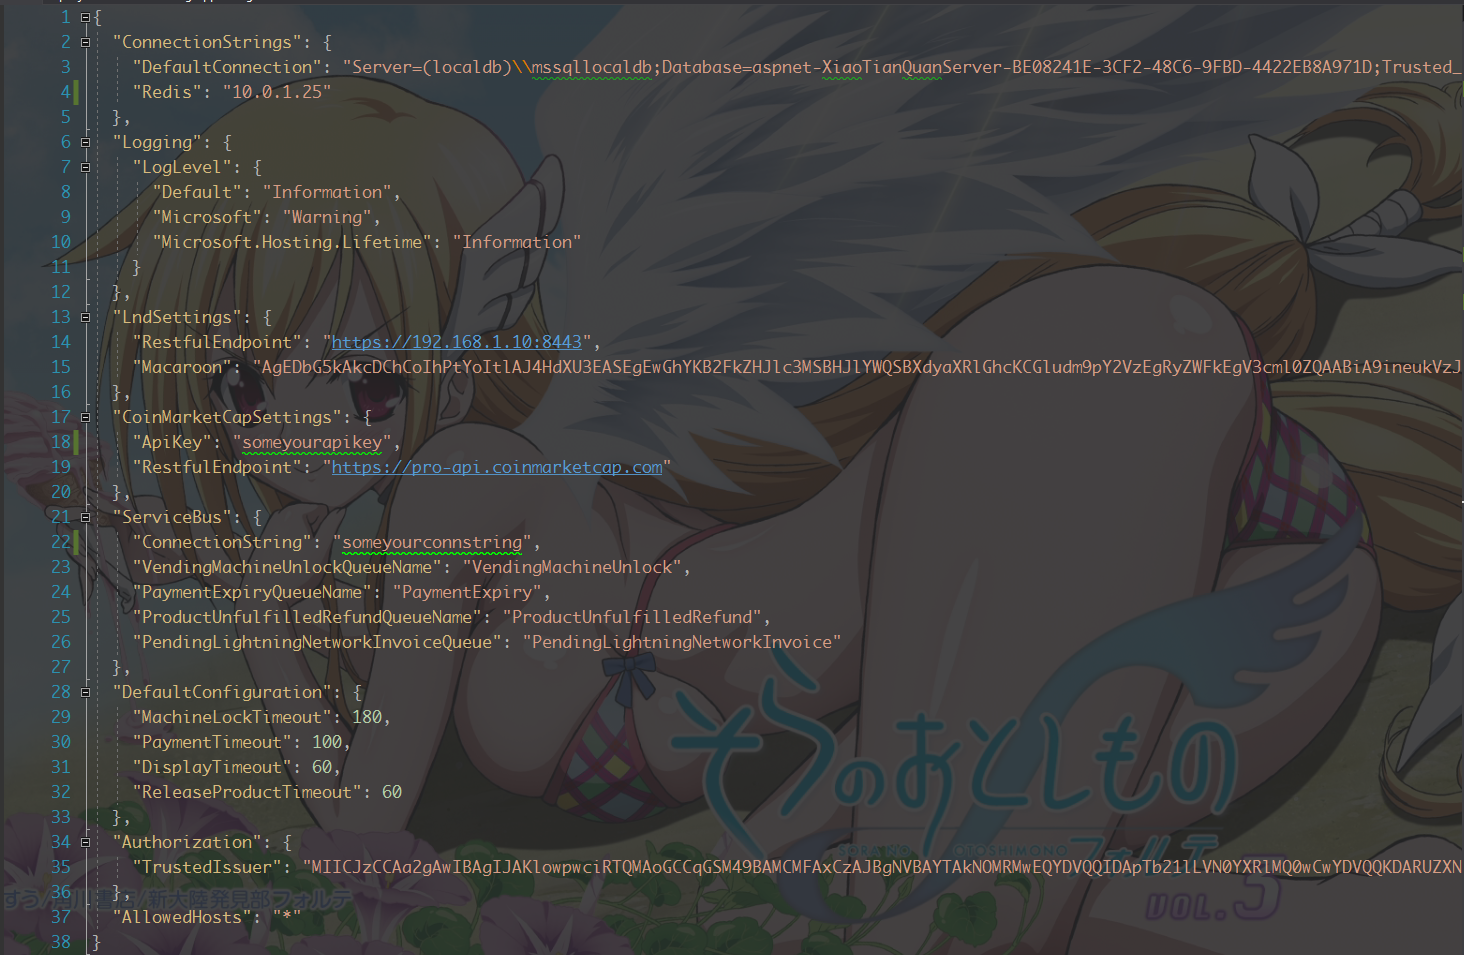
\includegraphics[width=\linewidth]{appsettings.png}
        \caption{服务器配置文件 appsettings.json}
        \label{fig:appsettings}
    \endminipage\hfill
    \end{figure}

\begin{itemize}
  \item ConnectionStrings
  \item LndSettings
  \item CoinMarketCapSettings
  \item ServiceBus
  \item DefaultConfiguration
  \item Authorization
\end{itemize}

\subsubsection{ConnectionStrings}

本节用以配置相关数据库连接的连接字符串。

\paragraph{DefaultConnection}


SQL Server的连接字符串。
    \begin{exmp}
        \begin{lstlisting}
            "DefaultConnection":
            "Server=(localdb)\\mssqllocaldb;
            Database=aspnet-XiaoTianQuanServer-BE08241E-3CF2-48C6-9FBD-4422EB8A971D;
            Trusted_Connection=True;MultipleActiveResultSets=true"
        \end{lstlisting}
    \end{exmp}

\paragraph{Redis}


Redis的连接字符串
    \begin{exmp}
        \begin{lstlisting}
            "Redis": "192.168.1.10"
        \end{lstlisting}
    \end{exmp}

\subsubsection{LndSettings}
本节用以配置Lightning network daemon相关

\paragraph{RestfulEndpoint}


Lnd的restful接口,请参阅lnd conf以确定
    \begin{exmp}
        \begin{lstlisting}
            "RestfulEndpoint": "https://192.168.1.10:8443"
        \end{lstlisting}
    \end{exmp}

\paragraph{Macaroon}


Lnd具备invoice权限用户的macaroon,请参阅\ref{sec:lnd-macroon}以取得该字串
    \begin{exmp}
        \begin{lstlisting}
            "Macaroon":
            "AgEDbG5kAkcDChCoIhPtYoItlAJ4HdXU3EASEgE
             wGhYKB2FkZHJlc3MSBHJlYWQSBXdyaXRlGhcKCG
             ludm9pY2VzEgRyZWFkEgV3cml0ZQAABiA9ineuk
             VzJNt7Tv9952AnCbLpYn1ElQ2tAO9RqVvamHg=="
        \end{lstlisting}
    \end{exmp}

\subsubsection{CoinMarketCapSettings}
本节用以配置CoinMarketCap的相关内容

\paragraph{ApiKey}


CoinMarketCap的ApiKey

\paragraph{RestfulEndpoint}


需要使用的CoinMarketCap restful endpoint,通常为https://pro-api.coinmarketcap.com

\subsubsection{ServiceBus}

本节用以配置Azure ServiceBus相关内容

\paragraph{ConnectionString}


Azure Service服务的连接字符串

\subsubsection{DefaultConfiguration}
本节用以配置服务器中的相关默认项

\paragraph{PaymentTimeout}


用户付款动作的超时时间

\paragraph{DisplayTimeout}


用户付款展示页面的超时时间,本时间需要小于PaymentTimeout

\paragraph{ReleaseProductTimeout}


机器释放货物的超时时间,超过此时间服务器若仍未收到货物释放的确认将会执行退款

\subsubsection{Authorization}
本节用以配置售货机连接服务器的相关鉴权设置

\paragraph{TrustedIssuer}


售货机连接的client SSL Certificate issuer

\subsection{数据库迁移}

如果数据库未做过迁移,请在完成了配置文件编写之后执行迁移。需要确保Redis服务已经启动并可连接,执行如下命令(此命令来自.Net Core SDK,操作详见附录\ref{sec:newdb}):
    \begin{verbatim}
        dotnet ef database update
    \end{verbatim}

您也可以通过导入SQL文件的形式完成数据库迁移,亦请见附录\ref{sec:newdb}。

\subsection{运行服务器}

完成了服务器配置之后,可以启动服务器。请首先启动依赖的服务再启动服务器。

在服务器软件目录下使用如下命令启动服务器:

    \begin{verbatim}
    dotnet XiaoTianQuanServer.dll
    \end{verbatim}

如果命令行没有报告任何错误,服务器即启动完成。

\subsection{服务器软件FAQ}

\subsubsection{我的服务器报告xxx错误,如何解决?}

\begin{verbatim}
fail: XiaoTianQuanServer.Services.LightningNetwork.LightningNetworkSubscribeService[0]
      invoice subscription request failed
      A connection attempt failed because the connected party did not properly
      respond after a period of time, or established connection failed because
      connected host has failed to respond.
      A connection attempt failed because the connected party did not properly
      respond after a period of time, or established connection failed because
      connected host has failed to respond.
\end{verbatim}

服务器未能与lnd建立连接,请检查lnd的端口设置与防火墙设置

\section{售货机软件}

\subsection{安装}

\textit{目前的安装流程较为复杂,我们正在优化该流程}

请确保您具有支持以下条件的Windows 10 IoT Core硬件设备\footnote{我们开发调试使用的是DragonBoard 410c,它亦是现阶段推荐的SoC}:
\begin{itemize}
  \item 支持TCP/IP访问售货机服务器,WiFi/Cellular/WiMax都可以
  \item 支持使用触摸屏设备
  \item 带有I2C模块
  \item 带有空余GPIO接口
\end{itemize}

同时您需要准备好以下软件:
\begin{itemize}
  \item Visual Studio 2019 w/ Universal Windows App development
\end{itemize}

首先请签出位于
\url{https://github.com/Andoromeda-Foundation/CryptoVendingMachineSoftware} 的售货机软件的代码。打开解决方案,找到VendingMachineKiosk项目。

\subsection{配置}\label{sec:vm-soft-config}

编辑\verb|Config.cs|文件以适应本机情况,如图\ref{fig:kioskconfig}所示。内含有三个字段,分别是
\begin{description}
  \item[RequestEndpoint] 售货机服务器的https端点
  \item[CertificateIssuer] 本售货机client SSL 证书的签发者CN,详见\ref{sec:ssl-cert:root}
  \item[ProductSelectionIdleTimeout] 用户商品选择页超时时间
\end{description}

    \begin{figure}[htbp]
    \minipage[b][][b]{\textwidth}
        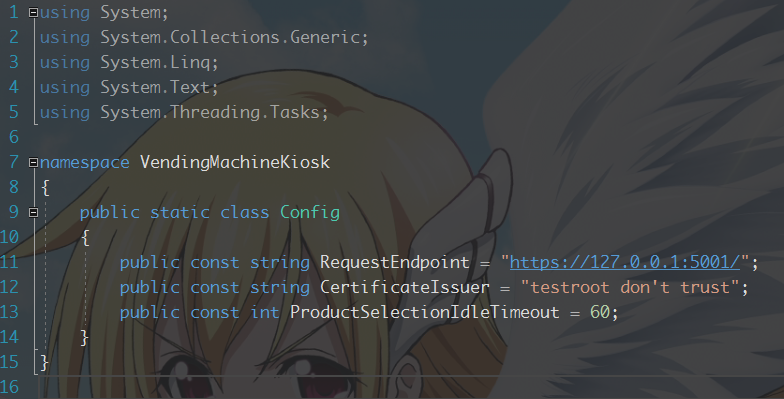
\includegraphics[width=\linewidth]{kioskconfig.png}
        \caption{售货机软件配置}
        \label{fig:kioskconfig}
    \endminipage\hfill
    \end{figure}

\subsection{部署}

完成编辑后,请编译该项目,并将Windows 10 IoT Core设备连接到该计算机。请在调试栏选择设备Remote Machine(图\ref{fig:remotemachine})。如果您是首次选择Remote Machine,会要求您选择相应设备,如图\ref{fig:remotemachineselection}。若auto detection中未出现该设备,请手动输入设备的IP地址。

部署该项目。如果一切正常,恭喜您,已经完成了售货机软件的部署。您亦可启动调试,这与Windows的远程调试体验是一致的。

    \begin{figure}[htbp]
    \minipage[b][][b]{\textwidth}
        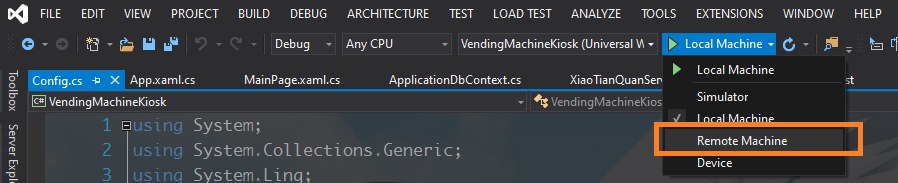
\includegraphics[width=\linewidth]{remotemachine.png}
        \caption{选择部署目标 Remote Machine}
        \label{fig:remotemachine}
    \endminipage\hfill
    \end{figure}

    \begin{figure}[htbp]
    \minipage[b][][b]{\textwidth}
        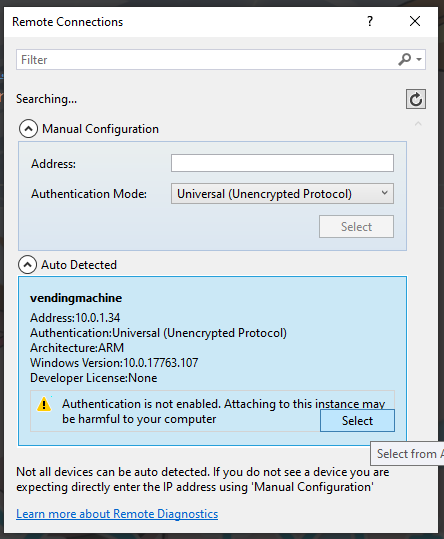
\includegraphics{remoteselection.png}
        \caption{选择 Remote Machine}
        \label{fig:remotemachineselection}
    \endminipage\hfill
    \end{figure}

\section{售货机硬件}

售货机硬件包含两部分,通用的应用板部分(即上一章的内容)已经适配不同售货机的控制板部分。我们在开发中,适配了百嵩实业的一款简易售货机。如果您有需要,可以自行定制售货机的控制板以适应不同的售货机硬件。

应用板与控制板通信采用I2C协议+ready信号。您可以参照 \\ \url{https://github.com/Andoromeda-Foundation/CryptoVendingMachineFirmware/blob/master/doc/control-protocol.pdf}设计自己的控制板,同时在有事件时拉高ready引脚的电平,即可无缝对接应用板。

\subsection{Wiring指南}

请参阅控制板的电路图,将控制板的I2C端口与应用板的I2C端口相接。同时,将ready端口与控制板的某个GPIO相接。


\appendix

\section{附录 - 建立数据库}\label{sec:newdb}

通常,我们获得的都是一个新的数据库。要建立服务器所需要的schema我们提供两种方式:使用EntityFramework Core Migration或直接导入SQL。

\subsection{EF Core Migration}
服务器软件提供了在新数据库中建立应有表项的功能。该功能需要安装.Net Core SDK 3.0,并且签出服务器的源码。请按照如下步骤进行:

\begin{enumerate}
  \item 安装 .Net Core 3.0 SDK,请参阅 \\ \url{https://dotnet.microsoft.com/download/linux-package-manager/debian10/sdk-3.0.100}
  \item 签出服务器源码,并进入服务器工程目录
  \item \textbf{请配置appsettings中的Redis服务器,服务器不会被使用,但是迁移过程中服务器会自动检查该连接字符串的有效性}
  \item 配置appsettings中的SQL Server连接字符串
  \item 安装dotnet ef工具 \verb|dotnet tool install --global dotnet-ef|
  \item 执行\verb|dotnet ef database update|
\end{enumerate}

命令示例请见图\ref{fig:ef-update}

    \begin{figure}[htbp]
    \minipage[b][][b]{\textwidth}
        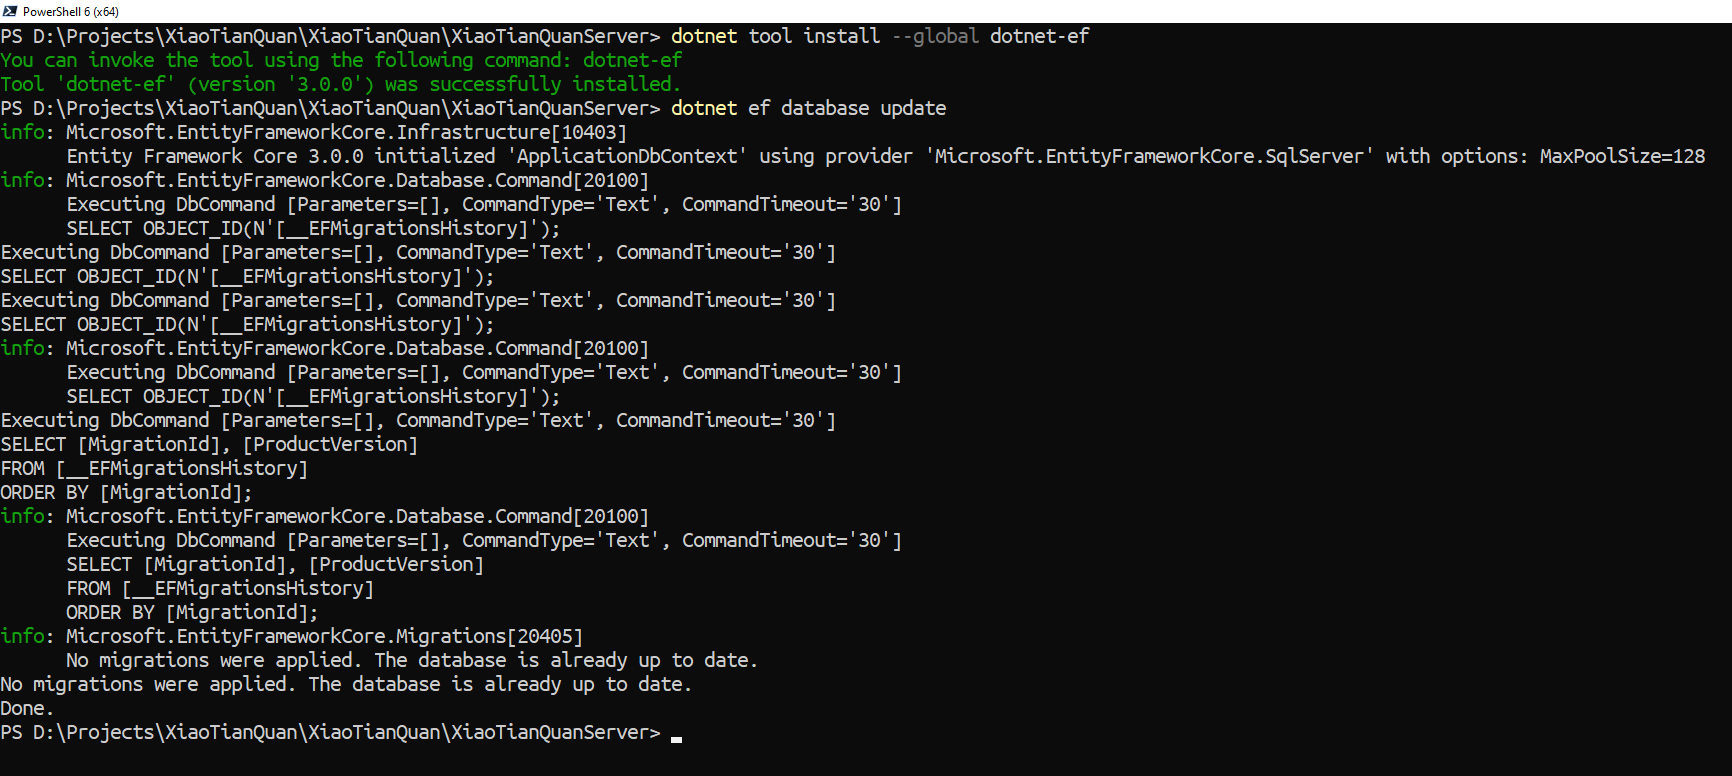
\includegraphics[width=\linewidth]{ef-update.png}
        \caption{执行 dotnet ef update}
        \label{fig:ef-update}
    \endminipage\hfill
    \end{figure}

\subsection{导入SQL}

请访问 \url{https://github.com/Andoromeda-Foundation/CryptoVendingMachineSoftware/releases} 以获得与服务器版本相同的 \verb|Migration.sql|文件。将此文件直接作为SQL导入数据库即可。

\section{附录 - 签发售货机client SSL证书}\label{sec:ssl-cert}

\emph{我们推荐您使用专业的工具签发client SSL证书。该指南仅提供基本的、调试用的证书生成方式。}

该指南需要使用openssl。

\subsection{生成售货机根证书}\label{sec:ssl-cert:root}

本节描述如何生成一个自签名的售货机根证书。请记录填写过的证书CN,\ref{sec:vm-soft-config}中的CertificateIssuer即为此CN,务必准确将其复制到配置中。

\begin{lstlisting}
# Generate secp384r1 ECC root private key
openssl ecparam -genkey -name secp384r1 >rootCA.key

# Generate a self-signed 10-year certificate with SHA-256 as digest
openssl req -x509 -new -nodes -key rootCA.key -sha256 -days 3650 -out rootCA.crt
\end{lstlisting}


\subsection{生成售货机证书}

本节描述如何生成一个被上一步生成的根证书签名的售货机证书。每一个售货机都需要一个唯一的证书,同时注意该证书的common name需要是售货机的ID (GUID)。

\begin{lstlisting}
# Generate secp384r1 ECC machine private key for vending machine 1
openssl ecparam -genkey -name secp384r1 >machine1.key

# Generate the certificate request for machine 1 with its private key
# CN *must* be GUID of the machine!!
openssl req -key machine1.key -new -out machine1.csr

# Sign the certificate request, making it a valid certificate for 10 years and SHA-256 digest
openssl x509 -req -in machine1.csr -CA rootCA.crt -CAkey rootCA.key -CAcreateserial -out machine1.crt -days 3650 -sha256
\end{lstlisting}

\subsection{将证书转换为PKCS\#12格式}

Windows下有时候处理PKCS\#12格式的证书会更加方便,此种证书密钥与证书部分包含在同一个文件内。使用以下命令以转换。

\begin{lstlisting}
# Export certificate as PKCS #12
openssl pkcs12 -in rootCA.crt -inkey rootCA.key -export -out rootCA.p12

openssl pkcs12 -in machine1.crt -inkey machine1.key -export -out machine1.p12
\end{lstlisting}

\subsection{获取服务器中需要的TrustIssuer}

appsettings.json中的TrustIssuer接受一个base64编码的x509证书字符串。执行如下指令并取得其输出:

\begin{lstlisting}
cat rootCA.crt | sed '1d;$d'  | tr -d '\n'
\end{lstlisting}


\cleardoublepage
% \phantomsection
\addcontentsline{toc}{section}{\listfigurename}
\listoffigures


\end{document}


















